%! TEX root = ../main.tex
\documentclass[main]{subfiles}

\begin{document}
\chapter{提案手法}
\label{chap:method}
% ここを書き換える: 提案手法の説明
\section{概要}
この章では，提案手法の全体像と各構成要素を説明する．
全体の流れは図を用いて示すと理解しやすい．
図\ref{fig:overview}に提案手法の処理の流れを示す\footnote{図は \texttt{figures/} に置く．TikZで描いた図は \texttt{figures/sample.tex} のように単体でPDFにしてから読み込む．}．

\begin{figure}[htbp]
  \centering
  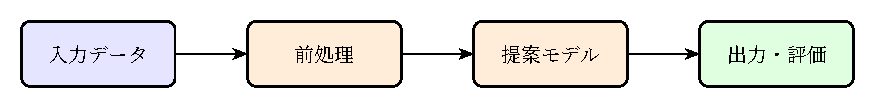
\includegraphics[width=120mm]{figures/sample.pdf}
  \caption{提案手法の処理の流れ．キャプションには，図だけを見ても内容が分かる程度の説明を書く．}
  \label{fig:overview}
\end{figure}

\section{定式化}
数式は \texttt{equation} 環境で書き，ラベルを付けて参照する．
例えば，入力 $\bm{x}$ に対するモデルの出力 $\hat{y}$ と正解 $y$ の二値交差エントロピー損失は式\eqref{eq:bce}で表される．
\begin{equation}
  \mathcal{L}(y, \hat{y}) = -\frac{1}{N} \sum_{i=1}^{N} \left\{ y_i \log \hat{y}_i + (1 - y_i) \log (1 - \hat{y}_i) \right\}
  \label{eq:bce}
\end{equation}
ここで，$N$ はサンプル数である．式中の記号は，初めて登場した箇所で必ず定義する．
\end{document}
